\documentclass[]{sigplan-proc}
\usepackage{graphicx}
\usepackage{epstopdf}
\usepackage{url}
\usepackage{listings}
\usepackage[colorlinks,urlcolor=blue]{hyperref}
\renewcommand{\topfraction}{0.85}
\renewcommand{\textfraction}{0.1}

\conferenceinfo{TBD}{TBD}
\CopyrightYear{2012}
\crdata{}

\begin{document}

\title{ A Study of Lustre Networking Over a 100 Gigabit Wide Area Network with 50 milliseconds of Latency}

\numberofauthors{3}
\author{
\alignauthor Scott Michael\\
	\affaddr{Indiana University}\\
	\affaddr{Bloomington, IN 47408}\\
	\email{scamicha@iu.edu}
\alignauthor Liang Zhen\\
        \affaddr{Whamcloud Inc.}\\
        \affaddr{Danville, CA 94526}\\
        \email{liang@whamcloud.com}
\alignauthor Robert Henschel\\
        \affaddr{Indiana University}\\
        \affaddr{Bloomington, IN 47408}\\
        \email{henschel@iu.edu}
\and
\alignauthor Stephen Simms\\
	\affaddr{Indiana University}\\
	\affaddr{Bloomington, IN 47408}\\
	\email{ssimms@indiana.edu}
\alignauthor Eric Barton\\
        \affaddr{Whamcloud Inc.}\\
        \affaddr{Danville, CA 94526}\\
        \email{eeb@whamcloud.com}
\alignauthor Matthew Link\\
	\affaddr{Indiana University}\\
	\affaddr{Bloomington, IN 47408}\\
	\email{mrlink@indiana.edu}		
}

\maketitle

\begin{abstract}

  As part of the SCinet Research Sandbox at the Supercomputing 2011 conference, Indiana University utilized a
  dedicated 100 Gbps wide area network (WAN) link spanning more than 3,500 km (2,175 mi) to demonstrate the
  capabilities of the Lustre high performance parallel file system in a high bandwidth, high latency WAN
  environment. This demonstration functioned as a proof of concept and provided an opportunity to study
  Lustre's performance over a 100 Gbps WAN. To characterize the performance of the network and file system a
  series of benchmarks and tests were undertaken. These included low level iperf network tests, Lustre
  networking (LNET) tests, file system tests with the IOR benchmark, and a suite of real-world applications reading
  and writing to the file system. All of the tests and benchmarks were run over a the WAN link with a latency
  of 50.5 ms. In this article we describe the configuration and constraints of the demonstration and focus in
  on the key findings and discoveries made regarding the Lustre networking layer for this extremely high
  bandwidth and high latency connection. Of particular interest is the relationship between the {\tt peer\_credits}
  and {\tt max\_rpcs\_in\_flight} settings when considering LNET performance.

\end{abstract}

\category{H.3.4}{Information Storage and Retrieval}{Systems and Software}[Distributed systems, Performance evaluation (efficiency and effectiveness)]
\category{C.2.2}{Computer-\linebreak Communication Networks}{Network Protocols}[Protocol architecture (OSI model),
Routing protocols]

\terms{Algorithms, Performance}

\keywords{WAN file systems, Lustre, Data Superconductor}

\section{Introduction}\label{sec:intro}

The SCinet Research Sandbox (SRS) at the Supercomputing 2011 (SC11) conference encourages institutions to
showcase new and innovative technologies in the area of networking. For the demonstration SCinet, in
collaboration with ESnet and Internet2, provided all SRS participants with a 100 Gbps network connection from
the SC11 show floor to the Internet2 backbone. This link provided an end-to-end connection from the IU booth
on the SC11 show floor to the IU Data Center in Indianapolis, Indiana. 

The overall goal of the IU entry into the SRS was to demonstrate the use of a Lustre file system in scientific
applications over the 100 Gbps wide area network (WAN) spanning from Seattle, Washington to Indianapolis,
Indiana, a distance in excess of 3,500 km (2,175 mi). A diagram of the network and routing points is given in
figure \ref{fig:network}. Such a use case is of obvious intrest for geographically distributed workflows; for
example, when data sources, such as remote sensors are in locations very distant from computational resources
used to analyze the data \cite{henschel2010}. Though the overall demonstration was ultimately successful, IU
achieved the highest reported throughput (6.2 GB/s) with scientific applications running across the WAN, the
focus of this article is the performance of and lessons learned about the Lustre networking layer, LNET.

\begin{figure*}[t]
\begin{center}
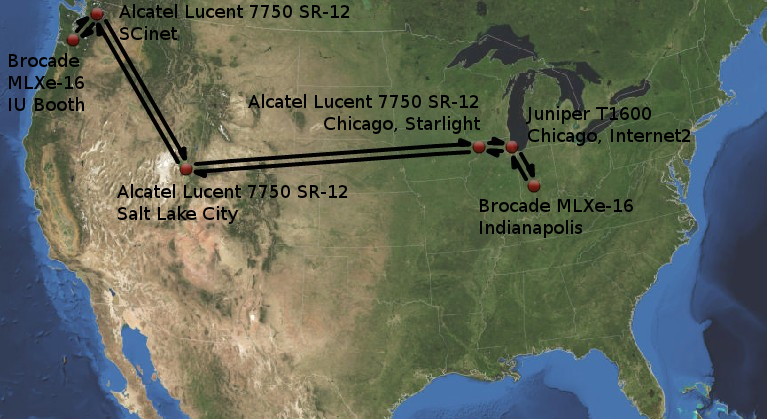
\includegraphics[width=0.80\textwidth]{figures/network.png}
\caption{Networking diagram for SRS demonstration. Routing points are labeled in the diagram.}
\label{fig:network}
\end{center}
\end{figure*}

Access to the 100 Gbps WAN was facilitated and coordinated by SCinet. Each participant was given time slots
for exclusive use of the network. The slots were evenly distributed from Saturday, November 12th to Thursday,
November 17th. In total, IU was provided nine test slots for a combined 16 hours. All testing that required
access to the network links had to be performed during those times, from setting up the actual end to end
network connectivity to performing file system and application tests. In addition, we were provided five
demonstration slots for a total of four hours. Those time slots were used to showcase the capabilities of the
system in the IU booth. All results described in this article were obtained in the 20 hours of demonstration
and test time.

The fact that this study was performed in such a limited timeframe influenced the measurements we were able to
take. In addition to the fact that the time allotted to IU was fairly short, the initial connection of the 100
Gbps link required some fine tuning of the routing elements between Seattle and Indianapolis to achieve an
eventual peak throughput of 96 Gbps on the TCP layer \cite{henschel2012}. Although the network issues were
eventually resolved, this phase of the troubleshooting consumed nearly half of the time allocated to IU,
leaving approximately 10 hours for troubleshooting and gathering data on LNET, file system benchmarks, and the
performance of  scientific applications.

This paper is structured as follows: Section \ref{sec:LNET} gives a brief technical overview of the LNET layer
of Lustre with particular attention paid to remote procedure calls (RPCs) and peer credits. Section
\ref{sec:usecase} describes in detail the SRS use case, including the hardware setup that was used for the SRS
demonstration and the particulars of the Lustre installation and software tools used. Section
\ref{sec:results} describes the results obtained from measurements of the Lustre networking layer. In section
\ref{sec:discussion} we offer some hypotheses explaining the results and compare to previous work. A summary and conclusion follows in section \ref{sec:conclusion}.

\section{The Lustre Networking Protocol}\label{sec:LNET}

The Lustre networking protocol (LNET) sits above the underlying network stack (e.g. TCP, IB, etc.) and
mediates the communication between Lustre components such as clients, servers, and metadata servers. 

{\bf COULD A MORE ACCOMPLISHED LNET EXPERT LIKE SIMMS, LIANG, OR BARTON ADD SOME MORE HERE?}

\subsection{Lustre Remote Procedure Calls}

The Lustre remote procedure call (RPC) mechanism allows one to send requests, receive and process requests,
perform bulk data transfer, and provide for error recovery. The number of outstanding RPCs that a single
client may submit to a single server is controlled by the Lustre tunable {\tt max\_rpcs\_in\_flight}. This is
a client-side setting and may be set on a per client basis. The default setting of {\tt max\_rpcs\_in\_flight}
= 8 may be suitable for many data center environments where there is relatively low latency between the
storage system and the clients it serves. However, in a WAN environment RTTs tend to be much longer and in
order to keep the maximum number of RPCs ``on the wire'' the {\tt max\_rpcs\_in\_flight} is typically
increased. Though one might think that raising the ceiling on RPCs should always improve performance, the
potential drawback lies in the fact that a single client can then consume more resources on a server, and at
some point, if {\tt max\_rpcs\_in\_flight} are increased across all clients, the server may become
overwhelmed. It should also be noted that the {\it Lustre Operations Manual} \cite{LustreManual2012} incorrectly
states that the largest value {\tt max\_rpcs\_in\_flight} may take is 32, when, in fact, we tested values up
to and including {\tt max\_rpcs\_in\_flight} = 256.

We are mainly concerned sends, receives, and bulk transfers because our LNET testing focused on bulk
operations. According to the {\it Understanding Lustre Internals} manual \cite{lustreint2009} a bulk transfer
operation requires two RPCs to complete. The minimum number of RPCs required to saturate a WAN link with a
given bandwidth delay product (BPD), obeys the following relationship.

\begin{equation}
\mathrm{RPCs > \frac{2\times BDP}{BS},}
\label{eq:rpcs}
\end{equation}
where RPCs is the {\it total} number of RPCs needed, and is a product of the Lustre tunable {\tt
  max\_rpcs\_in\_flight}, number of clients, and number of servers per client (i.e. stripes). BDP is the
bandwidth delay product given by, $\mathrm{link bandwidth \times RTT}$, and BS is the block size of the RPC
packets, typically 1 MB. This relationship has been seen previously by Simms et al. \cite{simms2007}, but was
not stated in this form. For the 100 Gbps link used in the SRS demonstration, with a 50.5 ms RTT and 1 MB
block size, slightly more than 5,000 RPCs are needed. 

\subsection{Lustre Peer Credits}

If one uses ksocklnd for the communication between Lustre network devices (LNDs) further tuning parameters
governing the amount of data ``on the wire'' are available within the ksocklnd module. The key parameters in
the case of the SRS demonstration, which we present results for in section \ref{sec:results}, were 
{\tt credits} and {\tt peer\_credits}. While the {\tt max\_rpcs\_in\_flight} parameter is applicable at a higher
layer, {\tt credits} and {\tt peer\_credits} control the number of messages that can be concurrently sent over
a LND network interface (NI). The {\tt credits} value determines the maximum number of {\it total} concurrent
sends from a NI, while the {\tt peer\_credits} value determines the maximum number of concurrent sends from a
NI to the same destination, or peer. By default {\tt credits} is set to 64 and {\tt peer\_credits} is set to
8. This means that a if single client stripes files over more than 8 servers using 8 {\tt peer\_credits} it
will exceed the number of allocated {\tt credits}. It should be noted that {\tt credits} and {\tt
  peer\_credits} apply to sends only, while {\tt max\_rpcs\_in\_flight} apply to both sends in
receives. Additionally, {\tt credits} and {\tt peer\_credits} are returned to their pool once the send is
completed and ``on the wire'', while RPCs can be outstanding for a longer period of time as they are not
retired until data hits the Lustre object storage target (OST).Due to these facts, one might expect
transactions to require a greater number of {\tt max\_rpcs\_in\_flight} than {\tt peer\_credits}.
 

\section {The SC11 Example Case}\label{sec:usecase}

As outlined in section \ref{sec:intro}, to showcase the capabilities of Lustre we set up a Lustre
file system and mounted it across the 100 Gbps cross-country WAN. To preform the demonstration we set up a
compute cluster on the show floor in Seattle and one in the IU data center in Indianapolis. We also deployed a
file system at each location. In addition, we installed and configured networking components to connect to the
Internet2/ESnet endpoints. The rest of this section details the hardware, network, Lustre, and other software
set up and configuration that was applied for the demonstration.

\subsection{Hardware}\label{sec:hardware}

Figure \ref{fig:hardwaresetup} shows the final hardware configuration that was used for the SRS demonstration. IBM provided 31 servers that functioned as compute nodes as well as the 16 storage servers that
were attached to the DataDirect Networks (DDN) storage devices. Brocade and Ciena provided the routing
equipment that enabled the network link from the show floor to Indianapolis.

The configurations of the compute cluster, storage, and networking components were identical in both
Indianapolis and Seattle. The central networking component at each endpoint was a Brocade MLXe-16 router that
provided a 100 Gbps Ethernet connection to the Ciena optical terminal managed by Internet2. The core router
also provided a 10 Gbps link to an IBM BNT G8264 OpenFlow enabled switch at each endpoint. The SRS
demonstration comprised a OpenFlow component in addition to the main Lustre 100 Gbps demonstration. However,
we will not discuss the OpenFlow component in this article. The 31 compute servers and 16 Lustre storage
servers were attached directly to the Brocade core router at 10 Gbps using Twinax cables and Brocade 1860
dual-port adapters.

The compute servers were IBM System x iDataPlex dx360 M3 systems, each configured with dual Intel Xeon E5645
6-core 2.40 GHz processors, 24 GB of DDR3 RAM, a Brocade 1860 adapter, and a 250 GB SATA hard drive. The
object storage servers (OSS) were IBM System x iDataPlex dx360 M3 servers each configured with an Intel Xeon
E5645 6-core 2.40 GHz processor, 48 GB of DDR3 RAM, a Brocade 1860 adapter, and a 1 TB SATA hard drive. The
OSS nodes at each site were connected directly to a DDN SFA10000 via 8 Gb Fibre Channel (FC). The metadata
server was identical to the compute servers, except it had 96 GB of RAM and was directly connected to a DDN
EF3015 RAID system that contained twelve 300 GB 15K RPM SAS disk drives for Lustre metadata. Due to space
constraints on the show floor server density was important. The throughput of the DDN SFA10000 allowed us to
use a single storage system for the Lustre OSS nodes at each site.

\begin{figure*}[t]
\begin{center}
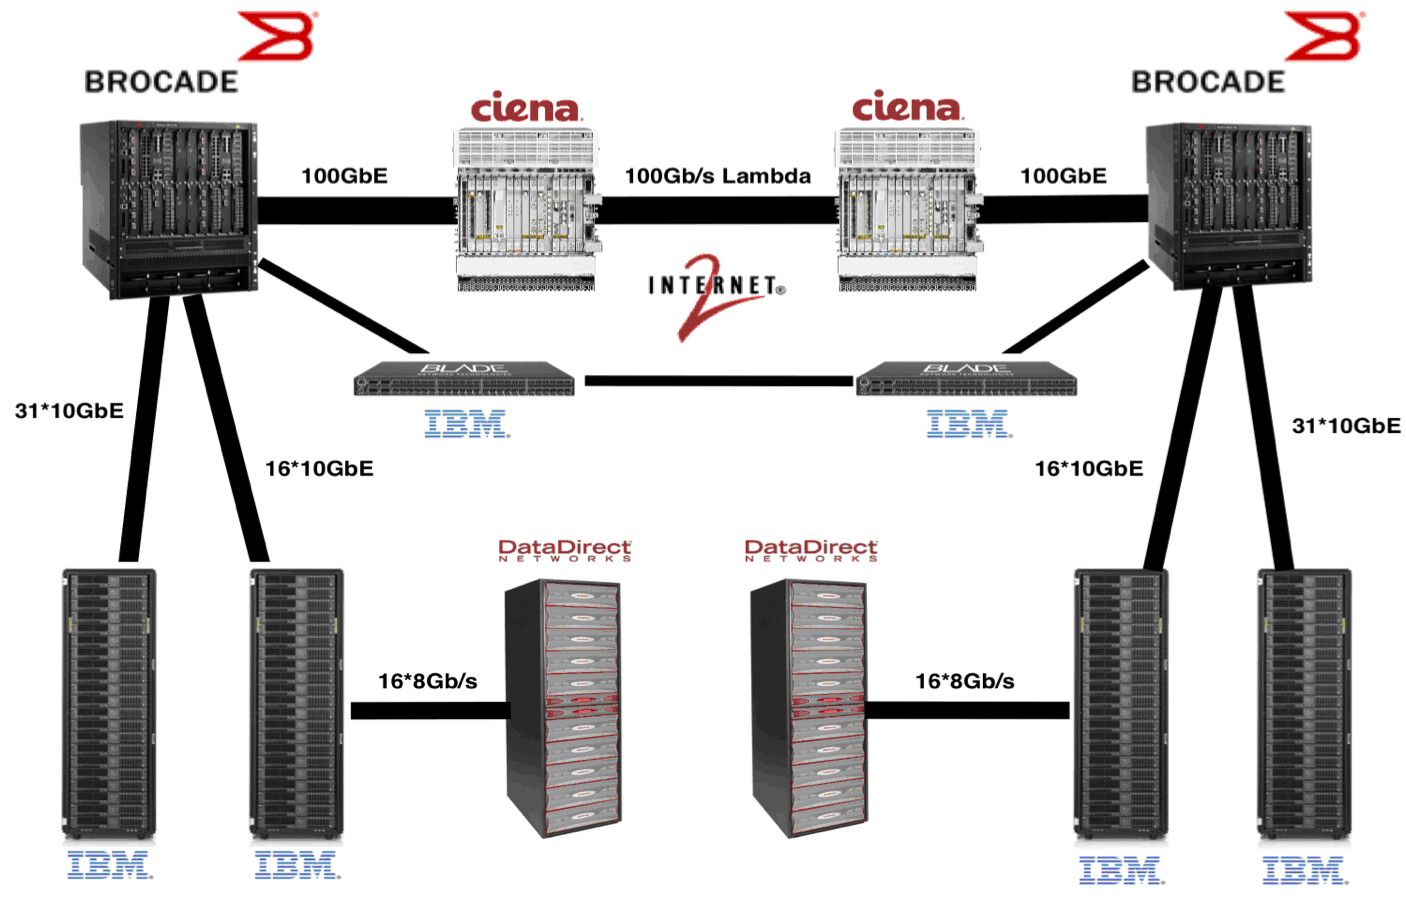
\includegraphics[width=0.80\textwidth]{figures/hardware.png}
\caption{Shown here is the hardware configuration used for the SRS demonstration. An IBM iDataPlex cluster and
  Lustre file system were connected to a Brocade 100 Gpbs MLXe-16 router at each endpoint. The IBM routing
  equipment connected to the Brocade routers was used for the OpenFlow component of the demonstration and is
  not discussed in this article. }
\label{fig:hardwaresetup}
\end{center}
\end{figure*}

\subsection{Network}

Before shipping equipment to the show floor in Seattle the demonstration configuration was assembled in the IU
machine room for testing.  There we performed tests with the two Brocade MLXe routers connected back to back
with the 100 Gbps connection spanning a few meters.  Local network tests across this connection showed a
latency of 0.24 ms and maximum stable performance of 98 Gbit/sec using TCP iperf \cite{iperf2012}.

The network link that was used for the SRS demonstration provided 100 Gbps connectivity from the IU booth on
the SC11 show floor to the IU Data Center in Indianapolis. In the months preceding the SC11 conference,
Indiana University worked with Internet2 to upgrade the existing link from Chicago to Indianapolis to 100
Gbps. For the SRS demonstration Internet2 and ESnet provided access to the 100 Gbps link from Chicago to Salt
Lake City and on to Seattle. From that point on to the show floor, SCinet was responsible for the network
link. The connection from Salt Lake City to Seattle had been established at 100 Gbps only two weeks prior to
SC11 and had undergone little to no performance testing.

Once the link was established, we measured a 50.5 ms round-trip time (RTT) between the clusters in Seattle and
Indianapolis. Initial TCP iperf tests showed good performance for two parallel streams, each at 10
Gbps. However, when adding more iperf streams to the link, performance dropped and throughput become
unstable. Working with Internet2, ESnet, and SCinet, we were able to tune several parts of the network and
achieve a stable 80 Gbps throughput with TCP iperf. Following all of our modifications, we were able to put a
stable 80 Gbps of TCP iperf traffic on the link by using 8 servers and clients. Unfortunately, adding another
single 10 Gbps stream to either of the connections resulted in congestion and degraded performance. However,
when oversubscribing the link by using all 30 compute nodes on each end, we were able to achieve a peak
throughput of 96 Gbps. Another unfortunate outcome was that the tuning steps yielded a stable connection only
in one direction, from Seattle to Indianapolis. We were never able to achieve similar results in the other
direction, and due to time constraints, we focused our efforts on just one direction.

\lstset{language=Bash, caption=Tuning parameters for the network, label=TuningListing}
\begin{lstlisting}
net.ipv4.tcp_rmem=4096 65536 167772160
net.ipv4.tcp_wmem=4096 65536 167772160
net.core.rmem_max=167772160
net.core.wmem_max=167772160
net.core.netdev_max_backlog=30000
eth2 txqueuelen 10000
eth2 mtu 9000
FlowControl off 
\end{lstlisting}

Listing \ref{TuningListing} shows the network tuning parameters that were set on all nodes. We increased the maximum TCP buffer to 167 MB and increased the sending and receiving queues to 10000 and 30000. In addtion, we enabled MTU 9000 and configured all nodes to use the \texttt{tcp\_bic} network stack. Flow control was disabled on the network adapters and the routers.

\subsection{Software and Lustre Configuration}

All of the clients and Lustre servers ran RedHat Enterprise Linux version XXXX. The Lustre servers used a
patched kernel with Lustre version XXX, while the clients used the patchless client version of Lustre with
version number XXX. Tests were conducted with the LNET self-test module that is part of the Lustre modules
toolkit. The LNET self-test scripts used to collect measurements for the SRS demonstration are available on
Github.com \cite{lstgithub2011}.

{\bf SIMMS NEED SOME ADDITIONAL STUFF HERE. MAYBE SHOULD OUTLINE THE OST CONFIG HERE?}

\section{Results}\label{sec:results}
\begin{equation}
\mathrm{Peak Bandwidth = \frac{RPCs \times BS}{2 \times RTT}}
\label{eq:band}
\end{equation}

\begin{figure}
\centering
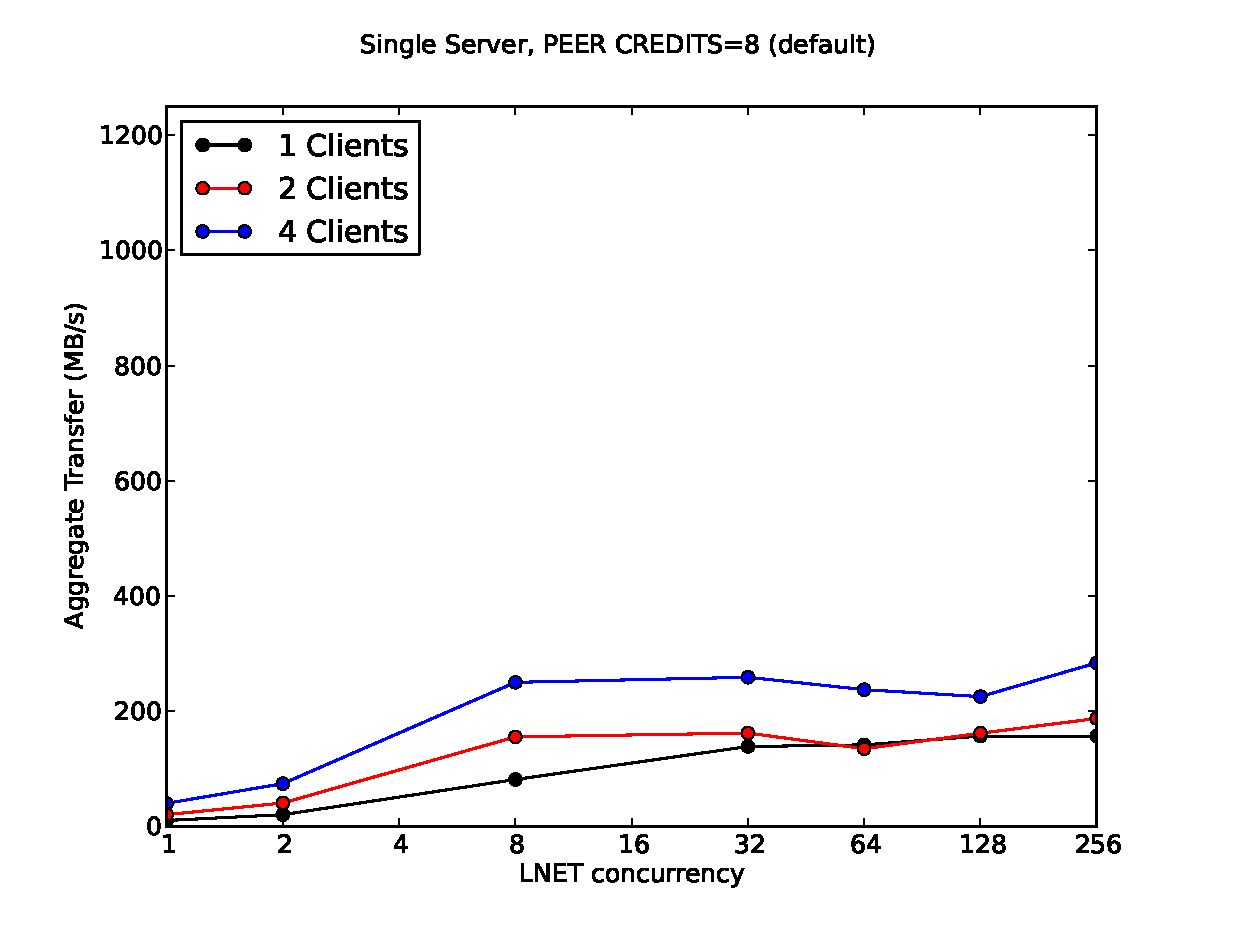
\includegraphics[width=0.50\textwidth]{figures/default_pc_plot.eps}
\caption{Results of LNET self test for 1, 2, and 4 clients using the default settings of 8 and 64 for {\tt
    peer\_credits} and {\tt credits}, respectively.}
\label{fig:default}
\end{figure}

\begin{figure}
\centering
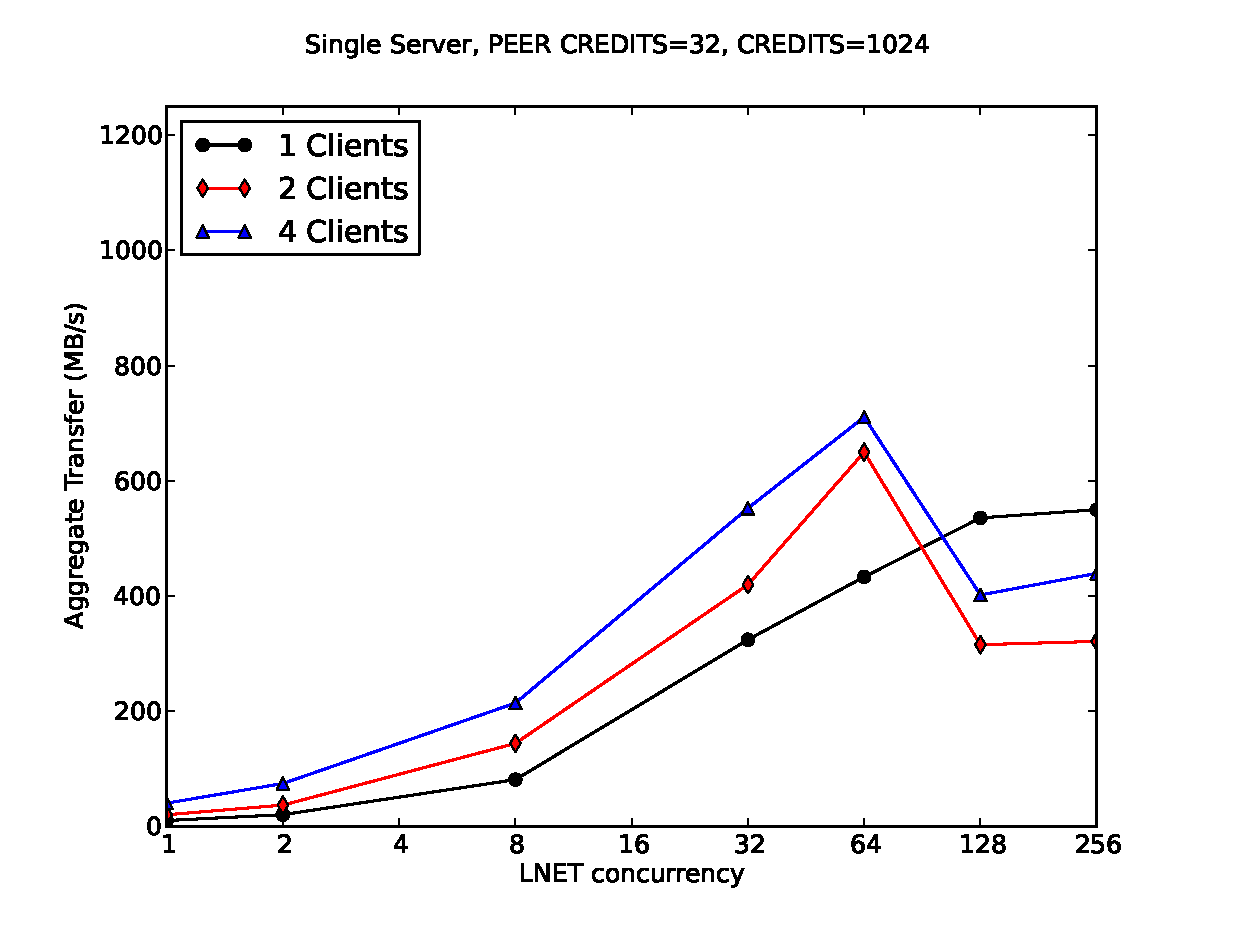
\includegraphics[width=0.50\textwidth]{figures/32pc_plot.eps}
\caption{Results of LNET self test for 1, 2, and 4 clients using the settings of 32 and XXX for {\tt
    peer\_credits} and {\tt credits}, respectively.}
\label{fig:32pc}
\end{figure}

\begin{figure}
\centering
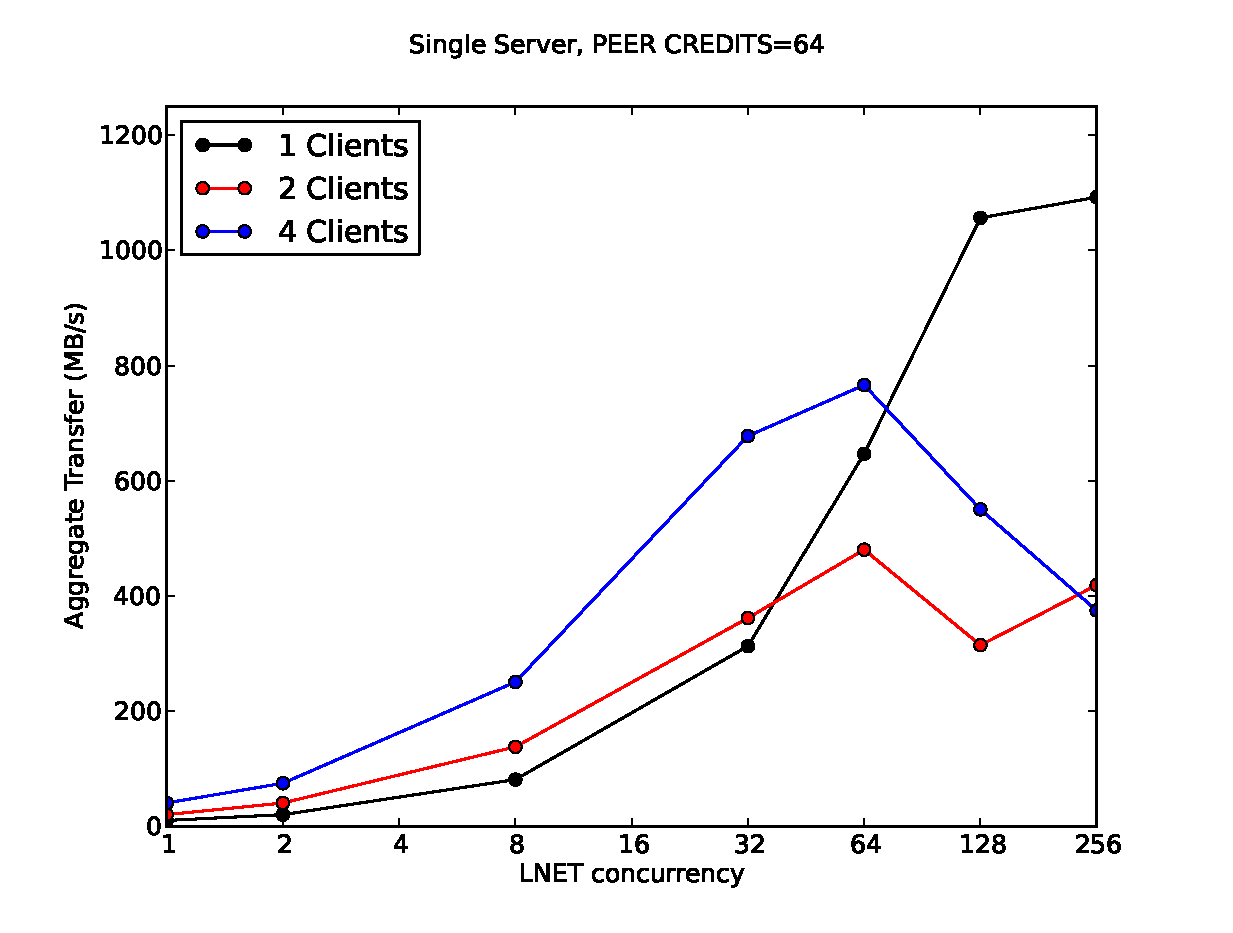
\includegraphics[width=0.50\textwidth]{figures/64pc_plot.eps}
\caption{Results of LNET self test for 1, 2, and 4 clients using the settings of 64 and XXX for {\tt
    peer\_credits} and {\tt credits}, respectively.}
\label{fig:64pc}
\end{figure}

\begin{figure}
\centering
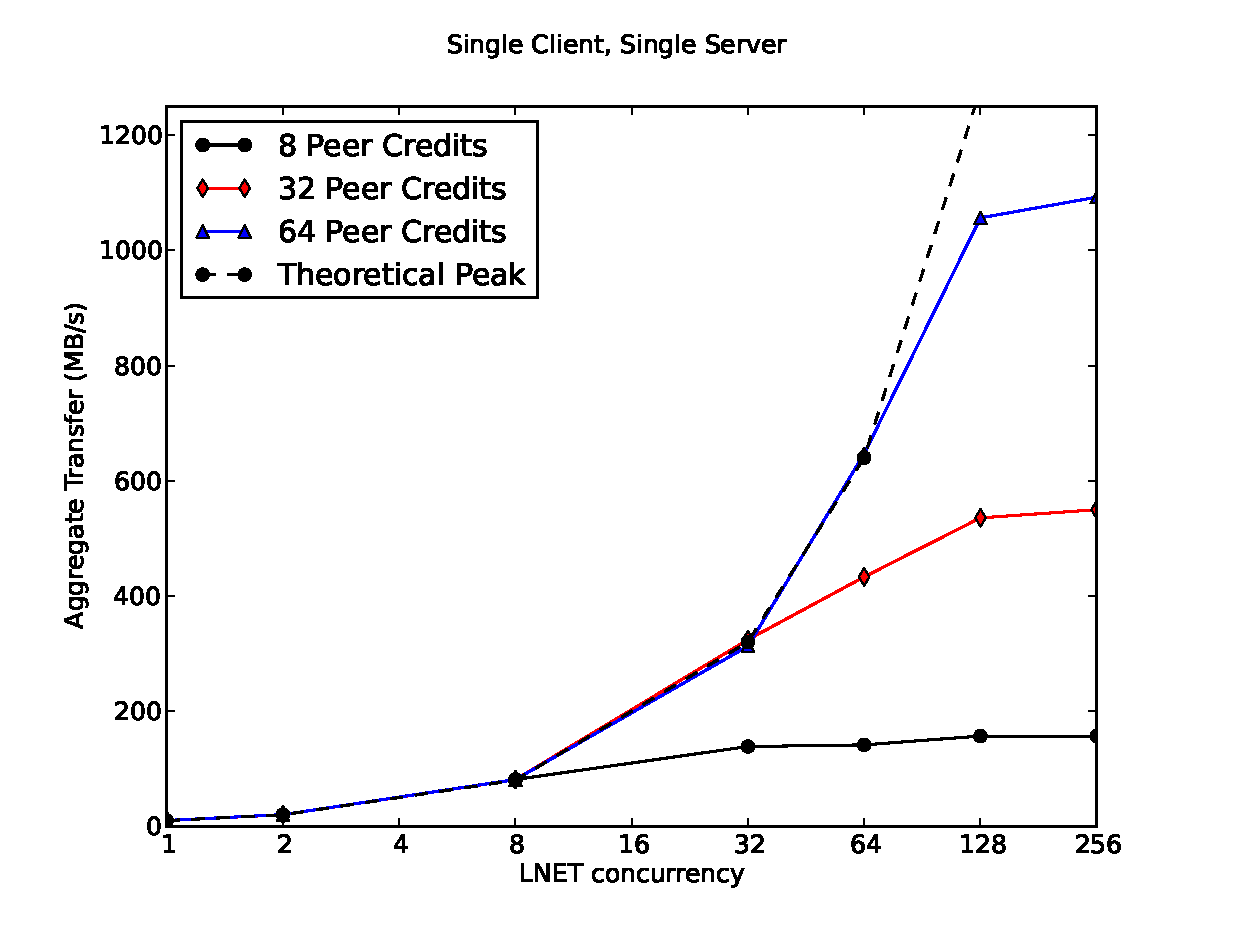
\includegraphics[width=0.50\textwidth]{figures/ss_plot.eps}
\caption{A comparison of single client, single server results of LNET self test for 8, 32, and 64 {\tt
    peer\_credits}. The values of {\tt credits} were set according to the {\tt peer\_credit} values. Also
  plotted is the theoretical peak throughput based on the number of RPCs as derived from equation \ref{eq:band}.}
\label{fig:singleserver}
\end{figure}

\begin{figure}
\centering
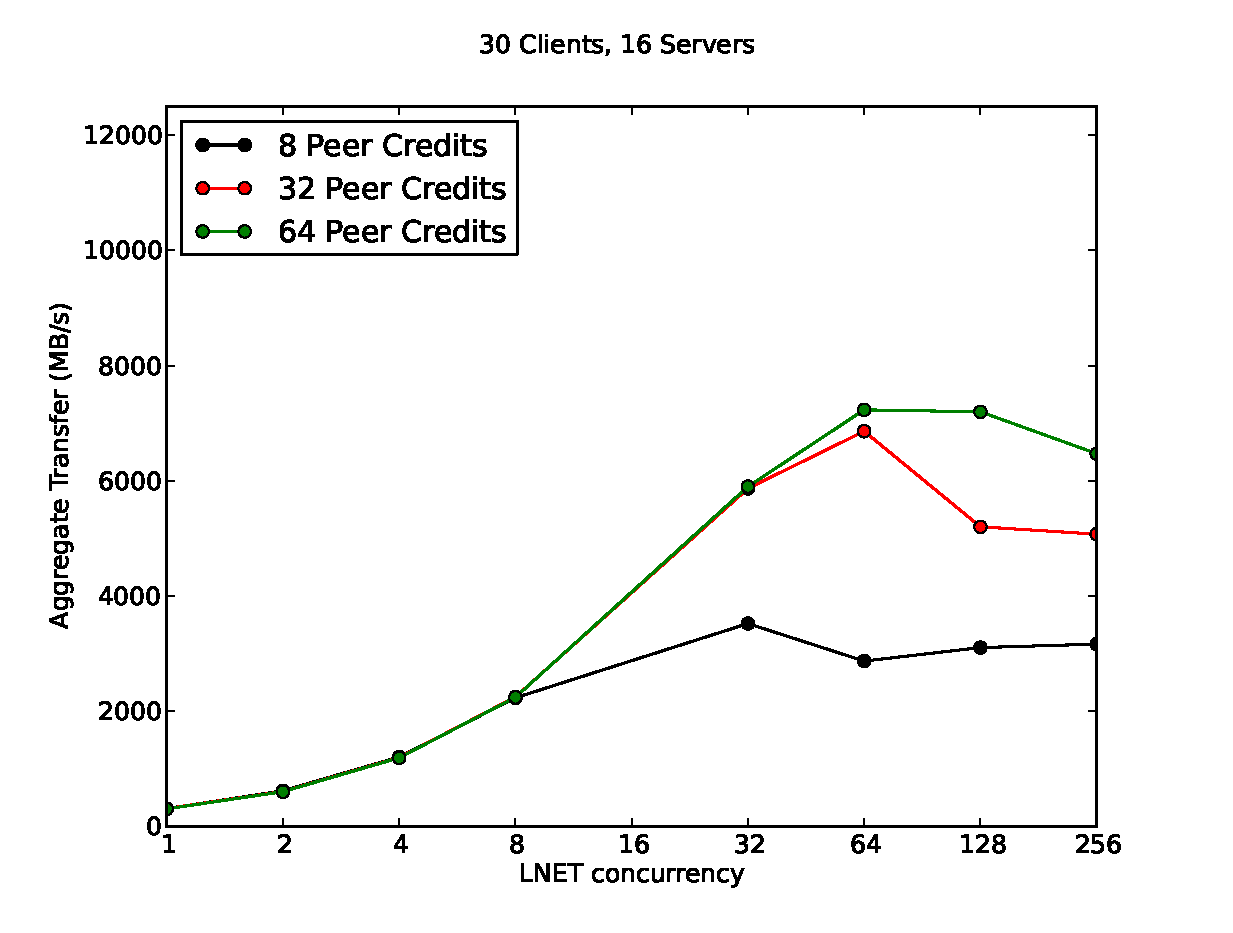
\includegraphics[width=0.50\textwidth]{figures/all_pc_plot.eps}
\caption{}
\label{fig:allserver}
\end{figure}

\section{Discussion}\label{sec:discussion} 

\section{Conclusions}\label{sec:conclusion}
  
\section{Acknowledgements}

The authors would like to thank the contributions of our collaborators and technical staff. The following
staff at IU provided excellent support in the administration of the systems, testing applications,
visualization, technical writing, and project management: Edward Balas, Janae Cummings, Kurt Seiffert, Daphne
Siefert-Herron, Bill Sherman, Martin Swany, Jenett Tillotson, George Turner, Matt Allen, Nathan Heald and Josh Walgenbach. Internet2 provided network setup and support: Andrew Lee, Chris Robb, and Matthew Zekauskas. ESnet staff also provided setup and troubleshooting assistance: Evangelos Chaniotakis and Patrick Dorn.

The following vendors provided loaner hardware to support this project: Brocade loaned all the server host
adapters, two MLXe-16 100 Gbps switches, required Fibre Channel and Ethernet optics, and all the Twinax cables
used to connect the servers to the network. Ciena loaned optical equipment to Internet2 to enable the 100 Gbps
network from Chicago to Seattle. DataDirect Networks loaned two SFA10000 storage systems for Lustre object
storage targets and two EF3015 RAID arrays for Lustre metadata storage. IBM contributed 22 iDataPlex dx360 M3
servers for the project as well as two OpenFlow enabled BNT G8264 switches with required optics. Internet2
provided networking equipment to extend their 100 Gbps network from Chicago to Indianapolis.

\bibliographystyle{abbrv}
\bibliography{LNET}
\end{document}
